\chapter{Modelo matemático}

De acuerdo con \cite[p.~14]{Dombre2007}, el diseño y control de robots requiere diversos modelos matemáticos, tales como:

\begin{itemize}
\item Cinemática directa e inversa, es decir, encontrar la posición del efector final en términos de las coordenadas de las articulaciones y viceversa.
\item Cinemática de la velocidad, encontrar la velocidad del efector final en términos de la velocidad de las articulaciones y viceversa.
\item Modelo dinámico, el cual establece la relación entre los torques o fuerzas que ejercen los actuadores y las posiciones, velocidades y aceleraciones de las articulaciones.
\end{itemize}

En este capítulo se desarrollarán estos modelos matemáticos, los cuales son necesarios para simular y predecir el comportamiento del mismo. 

Para realizar estos modelos, es necesario contar con los parámetros físicos y geométricos del robot, los cuales, para una primera aproximación se mencionarán a continuación.

Como podemos apreciar en el diagrama de requerimientos de la figura \ref{fig:requirementdiagram}, es necesario que el robot tenga seis grados de libertad del tipo revoluta, así, el diagrama de cuerpo libre de la cadena cinemática se expresa en la figura \ref{fig:kinematicchain}.

Otros requerimientos necesarios para el desarrollo del modelo matemático es el alcance total del brazo, el cual deberá ser de mínimo 450 mm, la velocidad, la cuál deberá estar en un rango entre 30\degree /s y 180\degree /s y la carga útil, que deberá ser de 2 kg.

\begin{figure}
    \centering
    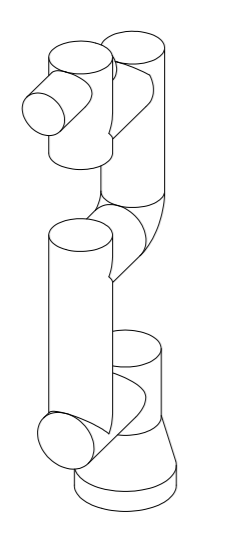
\includegraphics[scale=0.7]{./img/chapter4/robotarmprototype.png}
    \caption{Boceto del brazo robótico propuesto}
    \label{fig:roboticarmprototype}
\end{figure}

En la figura \ref{fig:roboticarmprototype} podemos ver un boceto del brazo robótico que se planea implementar.

Las distancias, masas e inercia de las articulaciones las podemos observar en la tabla x.

Con estos datos claros, es posible empezar la realización de los modelos matemáticos.

\section{Cinemática directa e inversa}
\subsection{Cinemática directa}
\subsubsection{Matriz de transformación homogénea}

\begin{figure}
    \centering
    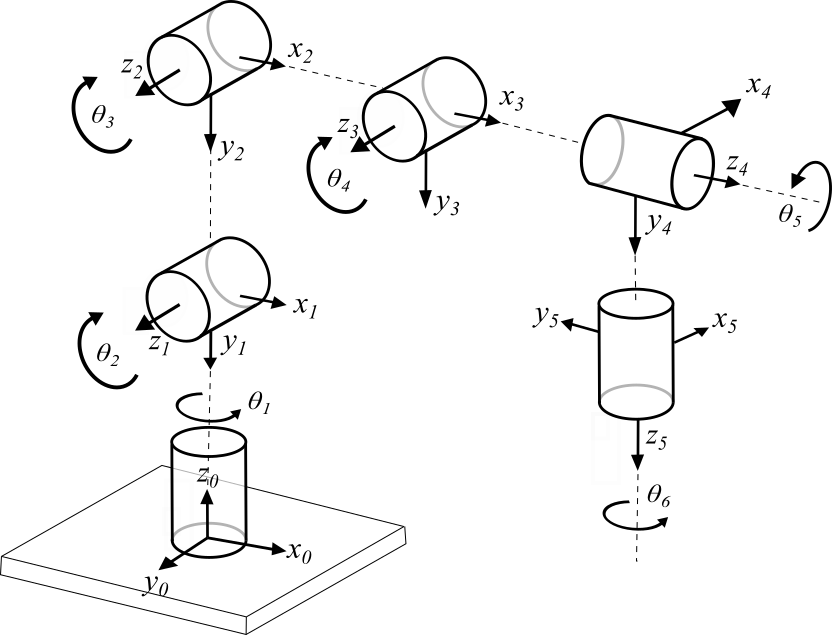
\includegraphics[width=\textwidth]{./img/chapter4/kinematicchainv5.png}
    \caption{Cadena cinemática ¿free body diagram?}
    \label{fig:kinematicchain}
\end{figure}

\[
{}_{0}^{1}T = 
\begin{bmatrix}
    1 & 0 & 0 & {a}_x  \\
    0 & \cos{\theta_1} & -\sin{\theta_1} & {a}_y \\
    0 & \sin{\theta_1} & \cos{\theta_1} & {a}_z \\
    0 & 0 & 0 & 1
\end{bmatrix}
\]

% Como no hay rotación en el frame, se usa la matriz identidad.

\[
{}_{1}^{2}T = 
\begin{bmatrix}
    1 & 0 & 0 & b_x  \\
    0 & 1 & 0 & b_y \\
    0 & 0 & 1 & b_z \\
    0 & 0 & 0 & 1
\end{bmatrix}
\]

% Como no hay rotación en el frame, se usa la matriz identidad.

\[
{}_{2}^{3}T = 
\begin{bmatrix}
    1 & 0 & 0 & c_x  \\
    0 & 1 & 0 & c_y \\
    0 & 0 & 1 & c_z \\
    0 & 0 & 0 & 1
\end{bmatrix}
\]

\[
{}_{3}^{4}T = 
\begin{bmatrix}
    \cos{\theta_4} & 0 & \sin{\theta_4} & d_x  \\
    0 & 1 & 0 & d_y \\
    -\sin{\theta_4} & 0 & \cos{\theta_4} & d_z \\
    0 & 0 & 0 & 1
\end{bmatrix}
\]

\[
{}_{4}^{5}T = 
\begin{bmatrix}
    1 & 0 & 0 & e_x  \\
    0 & \cos{\theta_5} & -\sin{\theta_5} & e_y \\
    0 & \sin{\theta_5} & \cos{\theta_5} & e_z \\
    0 & 0 & 0 & 1
\end{bmatrix}
\]

\[
{}_{0}^{5}T = {}_{0}^{1}T {}_{1}^{2}T {}_{2}^{3}T {}_{3}^{4}T {}_{4}^{5}T 
\]

\subsubsection{Convención de Denavit-Hartenberg}


\begin{table}[h]
\centering
\caption{Parámetros Denavit Hartenberg}
 \label{table:denavithartenberg}
\begin{tabular}{l|l|l|l|l|}
               & $\theta$ [rad] & a [m]    & d [m]   & $\alpha$ [rad]                        \\ 
\hline
Articulación 1 & 0                           & 0        & 0.1519  & $\frac{\pi}{2}$   \\
Articulación 2 & 0                           & -0.24365 & 0       & 0                                                  \\
Articulación 3 & 0                           & -0.21325 & 0       & 0                                                  \\
Articulación 4 & 0                           & 0        & 0.11235 & $\frac{\pi}{2}$   \\
Articulación 5 & 0                           & 0        & 0.08535 & $-\frac{\pi}{2}$  \\
Articulación 6 & 0                           & 0        & 0.0819  & 0                                                 
\end{tabular}
\end{table}

\subsection{Cinemática inversa}
No estoy seguro para que me servirá, si lo hará el software. MoveIt o MATLAB.

\section{Cinemática de la velocidad}


\section{Modelo dinámico}
\subsection{Formulación Lagraniana}
\subsection{Formulación Newton-Euler}